\chapter{Estudio de la interacción utilizando simulaciones Monte Carlo \label{chap:simulaciones}}
%%%%%%%%%%%%%%%%%%%%%%%%%%%%%%%%%%%%%%%%%%%%%%%%%%%%%%%%%%%%%%%%%%
%%%%%%%%%%%%%%%%%%%%%%%%%%%%%%%%%%%%%%%%%%%%%%%%%%%%%%%%%%%%%%%%%%
\noindent En este capítulo se presentan los resultados de modelar de forma cualitativa el proceso que se estudiará en esta tesis a partir de simulaciones Monte Carlo.


\section{Modelado del fenómeno físico}
\noindent Uno de los aspectos que se propuso estudiar en este trabajo es el de las razones físicas que hacen que el factor de Fano sea un número mucho menor que la unidad, al contrario de lo que podría esperarse desde una descripción puramente poissoniana de la interacción, donde el factor de Fano debería ser $1$.

Dado que el proceso de ionización de carga es un proceso estocástico en el cual un electrón ionizado (por ejemplo por efecto fotoeléctrico al interactuar con un fotón) puede o no interactuar con otros electrones de la red, puede pensarse como una serie de experimentos de Bernoulli, donde el \textit{éxito} es ionizar y generar otro par electrón-hueco y el \textit{fracaso} es no hacerlo. Como la probabilidad de ionización es baja, pero la cantidad de veces que puede darse la interacción es muy alta, en el límite el proceso es poissoniano. Sin embargo, experimentalmente se observa que cuando toda la energía de la partícula incidente es depositada en el material, el factor de Fano resulta casi un orden de magnitud menor\cite{TesisKevin}. Una de las posibles razones por las que esto sucede es que la energía de la partícula no solo es disipada en forma de ionización de carga, sino también en excitación de fonones de la red cristalina del material.

Cuando un fotón de alta energía cinética impacta contra el sensor, este produce una dispersión por ionización y emisión de fonones de la red cristalina del silicio, produciendo así una cascada de pares electrón-hueco. El número de pares producidos puede ser luego medido y el valor de la energía de creación electrón-hueco promediado a partir de este.

Este fenómeno es estudiando en los trabajos de R.C. Alig et al.\cite{Alig}, mediante simulaciones de Monte Carlo y luego por K. Ramanathan \cite{Ramanathan}, compilando resultados y propuestas de diferentes trabajos. En el primero se propone un modelo en el que la partícula incidente interactúa con el material, generando pares electrón-hueco por ionización en forma de cascada y, eventualmente, perdiendo energía por emisión de fonones. La forma en que la partícula incidente pierde energía depende fuertemente de la energía que tiene al momento de ionizar. Esta dependencia está modelada en el trabajo de Ramanathan\cite{Ramanathan} y lo llaman \textit{modelo simplificado}, donde proponen que la energía $E$ que se transfiere para generar pares electrón-hueco se reparte según una distribución Beta, de la forma
\begin{equation*}
    p(x|\alpha) = \frac{2}{B(\alpha)} x^{\alpha - 1}(1-x)^{\alpha - 1}
\end{equation*}
donde $x = \frac{E}{E_{R} - E_{g}}$ es la variable aleatoria, con $E_{r}$ la energía inicial de la partícula en cada ionización, $E_{g}$ es la energía del gap del silicio y $E$ la fracción de energía que va a parar a un nuevo par electrón-hueco. Utilizando esta distribución para generar realizaciones de la variable aleatoria $x$, se puede despejar el valor de $E$, que es la energía transferida para generar pares electrón-hueco según este modelo. Por otro lado, $B(\alpha)$ es la función Beta con un único parámetro $\alpha$, y viene dada por
\begin{equation*}
    B(\alpha, \beta) 
    = \frac{\Gamma(\alpha)\Gamma(\beta)}{\Gamma(\alpha) + \Gamma(\beta)}
    \longrightarrow
    B(\alpha)
    = \frac{\Gamma^{2}(\alpha)}{2\Gamma(\alpha)}
\end{equation*}
donde $\alpha$ depende de la energía $E_{r}$ y es el parámetro que determina el régimen de distribución de la energía, o en otras palabras, la forma de la distribución.

La motivación de la utilización de la distribución Beta para modelar cómo se reparte la energía en la generación de pares electrón-hueco por ionización se debe a que esta se adapta muy bien a los tres tipos de regímenes de energía en los que se puede encontrar la partícula incidente, según los trabajos mencionados anteriormente:
\begin{itemize}
    \item \textbf{A bajas energías de la partícula incidente}, se tienen distribuciones muy picudas en los extremos posibles: $E = 0$ y $E = E_{R}+E_{g}$,
    \item \textbf{A energías mucho mayores que la energía del gap}, $E_{R} >> E_{g}$: Se tiene una distribución aproximadamente uniforme,
    \item \textbf{A energías entre $2.2\,\si{eV}$ - $4.2\,\si{eV}$} se tiene una distribución de energía muy picuda en el medio de $x = E/(E_{R} - E_{g})$.
\end{itemize}
Para energías bajas, el parámetro $\alpha$ tiende a cero y se tiene una distribución con máximos en los extremos del intervalo. Para energías entre $2.2\,\si{eV}$ y $4.2\,\si{eV}$ se tiene una distribución con un máximo en el medio del intervalo y el parámetro $\alpha$ puede tender a infinito. Por último, para energías mucho mayores a la energía del gap, el parámetro $\alpha = 1$ y la distribución es uniforme. Estos casos se resumen en el gráfico de la Figura \ref{fig:BetaDist}.
\begin{figure}[h]
% Este gráfico se hace con el script que está acá: /home/igna/Escritorio/Tesis2021/Figs/Figuras_Apendice_Simulaciones/pys_para_plots DistBetaFig.py
    \centering
        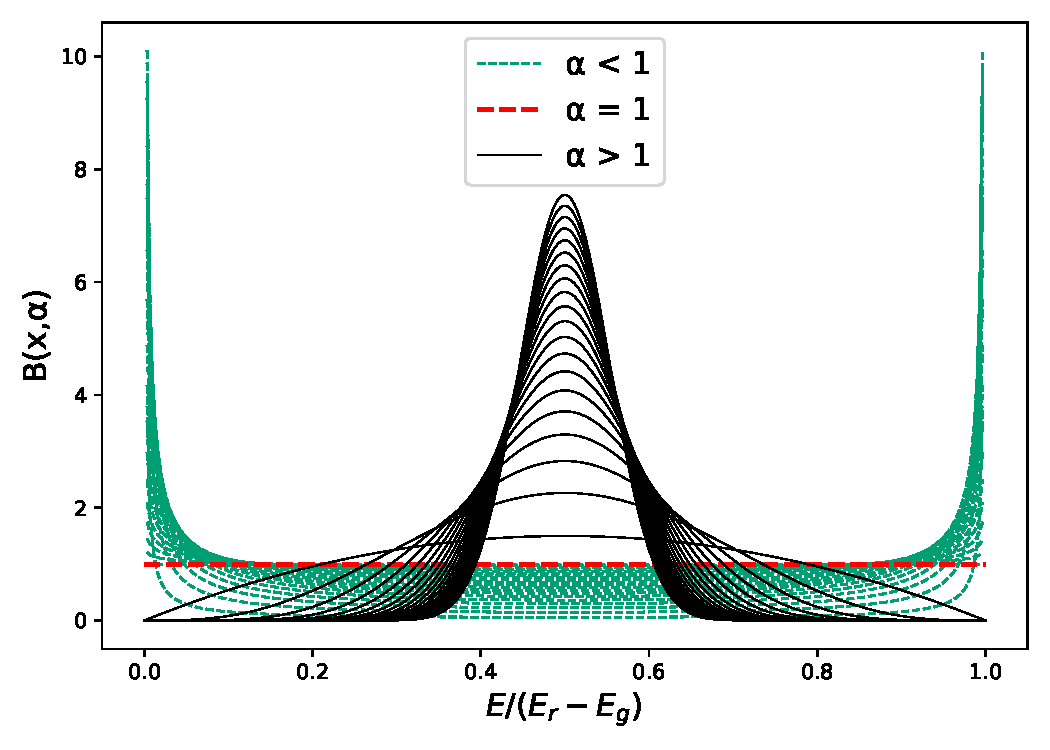
\includegraphics[scale=0.5]{Figs/BetaDistFig.pdf}
    \caption{Distribución Beta para diferentes valores del parámetro $\alpha$. Las curvas de trazo punteado son para $\alpha < 1$, la recta punteada es para $\alpha=1$ y las curvas de trazo continuo son para $\alpha>1$.}
    \label{fig:BetaDist}
\end{figure}

El mecanismo de cascada por el cual se producen las ionizaciones consiste en que para una dada energía inicial $E_{R}$, una fracción de esa energía se utiliza para generar un par electrón-hueco y la energía restante vuelve a fraccionarse para generar otros pares electrón-hueco. Estos pares generados, a su vez, utilizan fracciones de esa energía que les fue entregada para generar otros pares, en un proceso que se repite hasta que la energía disponible para repartir en cada rama de la cascada es menor a la energía del gap del Silicio y ya no es suficiente para generar más pares. Durante todo este proceso existe una probabilidad no nula de que parte de la energía se pierda por emisión fonones en la red.

Se define una probabilidad $P_{eh}$ para la cual se produce ionización y una probabilidad $1 - P_{eh}$ para la cual se produce emisión de fonones. Esta probabilidad depende de la energía inicial, al igual que el parámetro $\alpha$ de la distribución Beta, y viene dada por
\begin{equation}
    P_{eh}(E_{R}) = 
    \left[
        1 + \frac{\Gamma_{ph}(E_{R})}{\Gamma_{eh}(E_{R})}
    \right]^{-1}
        \label{ec:ProbabilidadIonizacion}
\end{equation}
donde 
\begin{equation*}
    \frac{\Gamma_{ph}(E_{R})}{\Gamma_{eh}(E_{R})}
    = A\frac{105}{2\pi}\frac{(E_{R} - \hbar \omega_{0})^{1/2}}{(E_{R} - E_{g})^{7/2}}
\end{equation*}
con $A = 5.2\,\si{eV^{3}}$, que es una constante fenomenológica que contiene información microscópica del sistema y que además puede ajustarse para reproducir valores medidos experimentalmente. Por otro lado, $\Gamma_{ph}$ y $\Gamma_{eh}$ son las tasas de producción de fonones y pares electrón-hueco, respectivamente. A partir de estos modelos, se buscó simular este mecanismo de ionización mediante simulaciones Monte Carlo.
%%%%%%%%%%%%%%%%%%%%%%%%%%%%%%%%%%%%%%%%%%%%%%%%%%%%%%%%%%%%%%%%%%
%%%%%%%%%%%%%%%%%%%%%%%%%%%%%%%%%%%%%%%%%%%%%%%%%%%%%%%%%%%%%%%%%%
\section{Simulaciones básicas}
\noindent El modelo más simplificado del mecanismo de ionización puede pensarse como una serie de experimentos de Bernoulli, es decir, donde solo hay dos resultados posibles: éxito-fracaso. La probabilidad de éxito $p$, representa la de ionizar una carga y perder una cantidad de energía equivalente a la energía de creación electrón-hueco, sin tener en cuenta explícitamente la disipación de energía por excitación de fonones.

Dada una energía inicial y un número fijo $N$ de experimentos de Bernoulli, puede suceder que la energía inicial se agote completamente o no. El valor final de la energía depende muy fuertemente del valor de $N$: para una cantidad de experimentos $N$ muy grande, la probabilidad de que la energía se agote completamente tiende a $1$, mientras que para $N$ muy pequeño la probabilidad es mucho menor, pudiendo suceder que la energía no sea cero al final del experimento. No es sorprendente que al simular con este modelo se recupere un factor de Fano que tiende a $1$, en el caso en el que el valor de $N$ es grande pero no suficiente para agotar la energía de la partícula incidente. Esto es debido a que la realización de experimentos consecutivos de Bernoulli conforman una variable aleatoria de distribución binomial, la cual tiende a una distribución de Poisson si además $p$ es pequeño. 
\begin{figure}[h]
%Para hacer este gráfico hay que correr el script que está en esta carpeta /home/igna/Escritorio/Tesis2021/Figs/Figuras_Apendice_Simulaciones/pys_para_plots y se llama Orden0_simu_SI_atraviesa.py con los datos de esta carpeta /home/igna/Escritorio/Tesis2021/Figs/Figuras_Apendice_Simulaciones/txts_para_plots y se llama orden0_simu_SI_atraviesa.txt
    \centering
    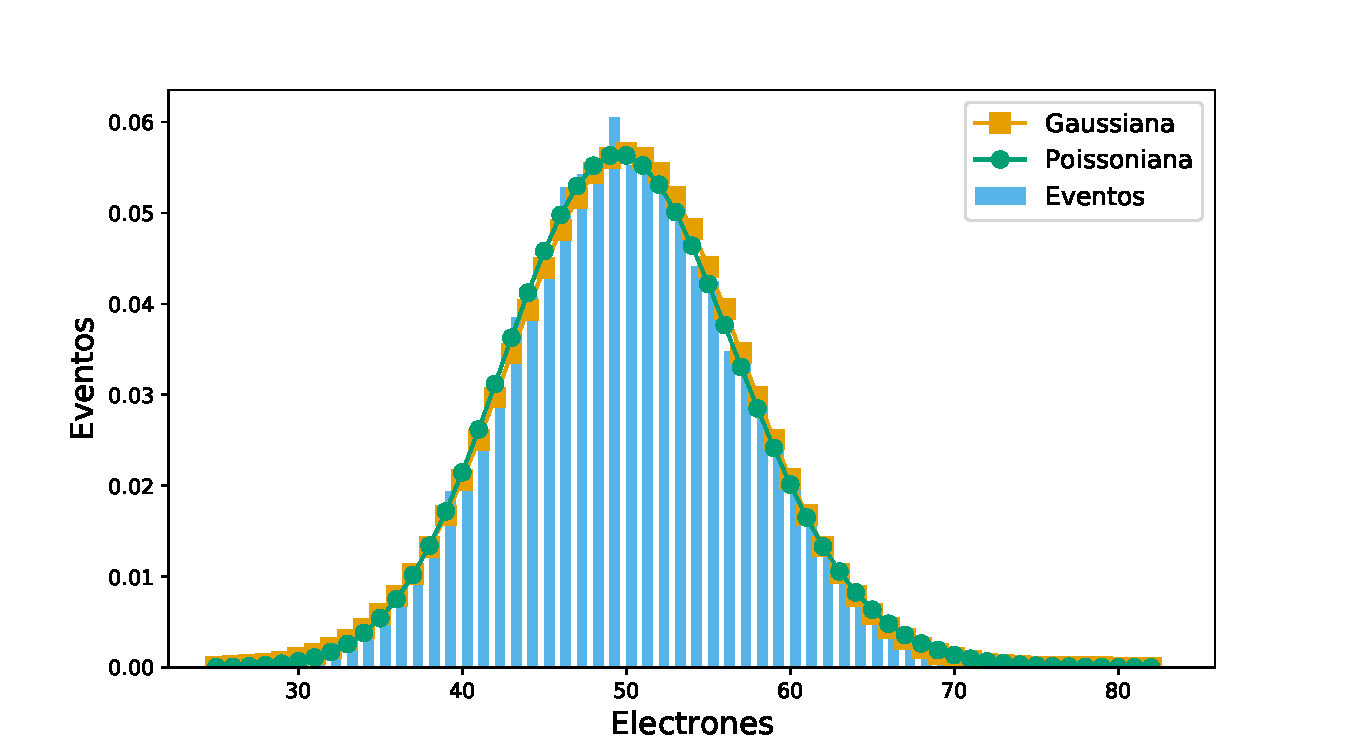
\includegraphics[scale=0.5]{Figs/Orden0_fano1.pdf}
    \caption{Histograma, con los correspondientes ajustes, gaussiano y poissoniano, de los resultados de $20000$ repeticiones, cada uno de los cuales consiste de $N = 5000$ experimentos de Bernoulli. En este caso la energía final de la partícula no es cero, es decir, la partícula incidente logra atravesar el material. Puede verse como el ajuste poissoniano representa muy bien al histograma de carga.}
    \label{fig:SimulacionOrden0Fano1}
\end{figure}
Esto puede verse en la Figura \ref{fig:SimulacionOrden0Fano1}, donde puede observarse como una distribución poissoniana describe correctamente el histograma. El histograma corresponde a la distribución de carga obtenida luego de repetir $20000$ veces la simulación, que parte de una energía inicial de $677\,\si{eV}$ con un $N = 5000$, que es la cantidad de veces que se repite el experimento de Bernoulli de ionizar o no con probabilidad $p=0.01$ y el factor de Fano resultó $F = 0.9790 \pm 0.0104$ mientras que el valor medio de eventos ionizados fue $\mu = 49.71 \pm 0.06$.

En oposición a lo previamente descripto, para el caso en que $N$ es tal que la gran mayoría de las veces la energía se agota completamente, el factor de Fano se vuelve menor a $1$, como puede verse en la Figura \ref{fig:SimulacionOrden0Fano0}. En este caso, nuevamente se parte de una energía inicial de $677\,\si{eV}$ pero esta vez con un $N = 30000$, cantidad suficiente para agotar completamente la energía y $p=0.01$ nuevamente. Esto se repitió $20000$ veces para obtener una buena cantidad de estadística y formar el histograma. En este caso el factor de Fano fue de $F = 0.2952 \pm 0.0025$ y el valor medio de carga ionizada $\mu = 200.97 \pm 0.06$.
\begin{figure}[h]
%Para hacer este gráfico hay que correr el script que está en esta carpeta /home/igna/Escritorio/Tesis2021/Figs/Figuras_Apendice_Simulaciones/pys_para_plots y se llama Orden0_simu_NO_atraviesa.py con los datos de esta carpeta /home/igna/Escritorio/Tesis2021/Figs/Figuras_Apendice_Simulaciones/txts_para_plots y se llama orden0_simu_NO_atraviesa.txt
    \centering
    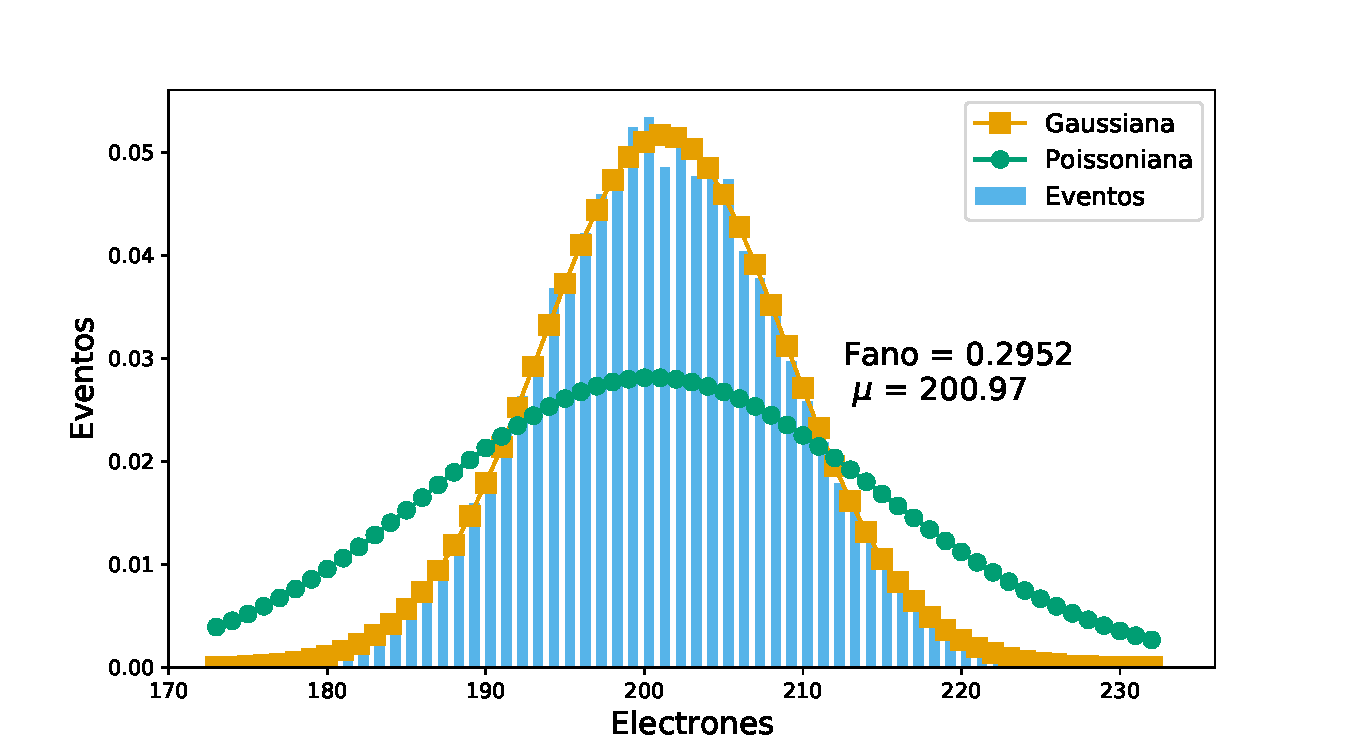
\includegraphics[scale=0.5]{Figs/Orden0_fano0.pdf}
    \caption{Histograma, con los correspondientes ajustes, gaussiano y poissoniano, de los resultados de $20000$ repeticiones, cada uno de los cuales consiste de $N = 30000$ experimentos de Bernoulli. En este caso la energía final de la partícula es casi siempre cero, es decir, la partícula incidente pierde toda su energía dentro del material. Es en este caso en el que el factor de Fano es menor a la unidad.}
    \label{fig:SimulacionOrden0Fano0}
\end{figure}

Si bien este modelo de juguete es una simplificación del proceso de dispersión real, los resultados soportan la hipótesis de que el factor de Fano es menor a $1$ debido, en parte, a que la partícula incidente deposita toda su energía en el material.
%%%%%%%%%%%%%%%%%%%%%%%%%%%%%%%%%%%%%%%%%%%%%%%%%%%%%%%%%%%%%%%%%%
%%%%%%%%%%%%%%%%%%%%%%%%%%%%%%%%%%%%%%%%%%%%%%%%%%%%%%%%%%%%%%%%%%
\section{Simulación de ionización en cascada}
\noindent Utilizando ideas tomadas de los trabajos anteriormente citados, se modificaron las simulaciones Monte Carlo con la intención de reproducir el mecanismo de creación de pares electrón-hueco por ionización en cascada. Para este caso se tuvo en cuenta la posibilidad de disipación de energía por emisión de fonones, a una energía fija de $\hbar\omega_{0} = 0.063\,\si{eV}$.

El resultado de la simulación es simplemente el número de pares 
ionizados a partir de la energía inicial $E_{R}$. De esta puede verse la distribución de la cantidad de pares generados y además calcular tanto su varianza como su esperanza, para así obtener el factor de Fano y la energía de creación electrón-hueco.
%Otro elemento a tener en cuenta en la simulación es la conservación de la energía durante el proceso de creación de pares. Puede considerarse que la energía transferida al ionizar es utilizada totalmente para ionizar otros pares o puede considerarse que siempre que se dé una ionización habrá una pequeña parte de energía que se pierde y no puede ser utilizada, es decir, que no se conserva la energía. 
Cabe destacar que en este tipo de simulación, dada su implementación particular, solo se puede considerar el caso en que la partícula disipa toda su energía en el interior del material, de modo que se esperan valores para el factor de Fano menores a la unidad.

Se realizaron las simulaciones partiendo de una energía inicial $E_{r} = 677\,\si{eV}$ y $E_{R} = 1500\,\si{eV}$, correspondiente a los rayos $X$ de flúor y del aluminio respectivamente, que son el principal objeto de estudio de este trabajo. Los valores de los parámetros fueron extraídos de la bibliografía\cite{Alig, Ramanathan} y son $A = 5.2\,\si{eV}^{3}$, la energía del gap $E_{g} = 1.1\,\si{eV}$, la energía de creación electrón-hueco promedio $\varepsilon_{eh} = 3.75\,\si{eV}$ y la energía perdida cada vez que se emiten fonones $\hbar \omega = 0.063\,\si{eV}$.

Por otro lado, con el fin de observar como afecta el número de repeticiones del experimento a la dispersión de los valores del factor de Fano, se realizó en primera instancia un barrido en la cantidad de repeticiones, partiendo desde $100$ hasta $100900$ repeticiones. En la Figura \ref{fig:FanoConvergencia} se observa la convergencia de los valores del factor de Fano a medida que aumenta el número de experimentos, para el caso de la energía de los rayos $X$ del flúor, $E_{R} = 677\,\si{eV}$.
\begin{figure}[h]
%Este gráfico se puede hacer con el script GrafFanoConvergencia.py que esta en este directorio /home/igna/Escritorio/Tesis2021/Figs/Figuras_Apendice_Simulaciones/pys_para_plots
    \centering
    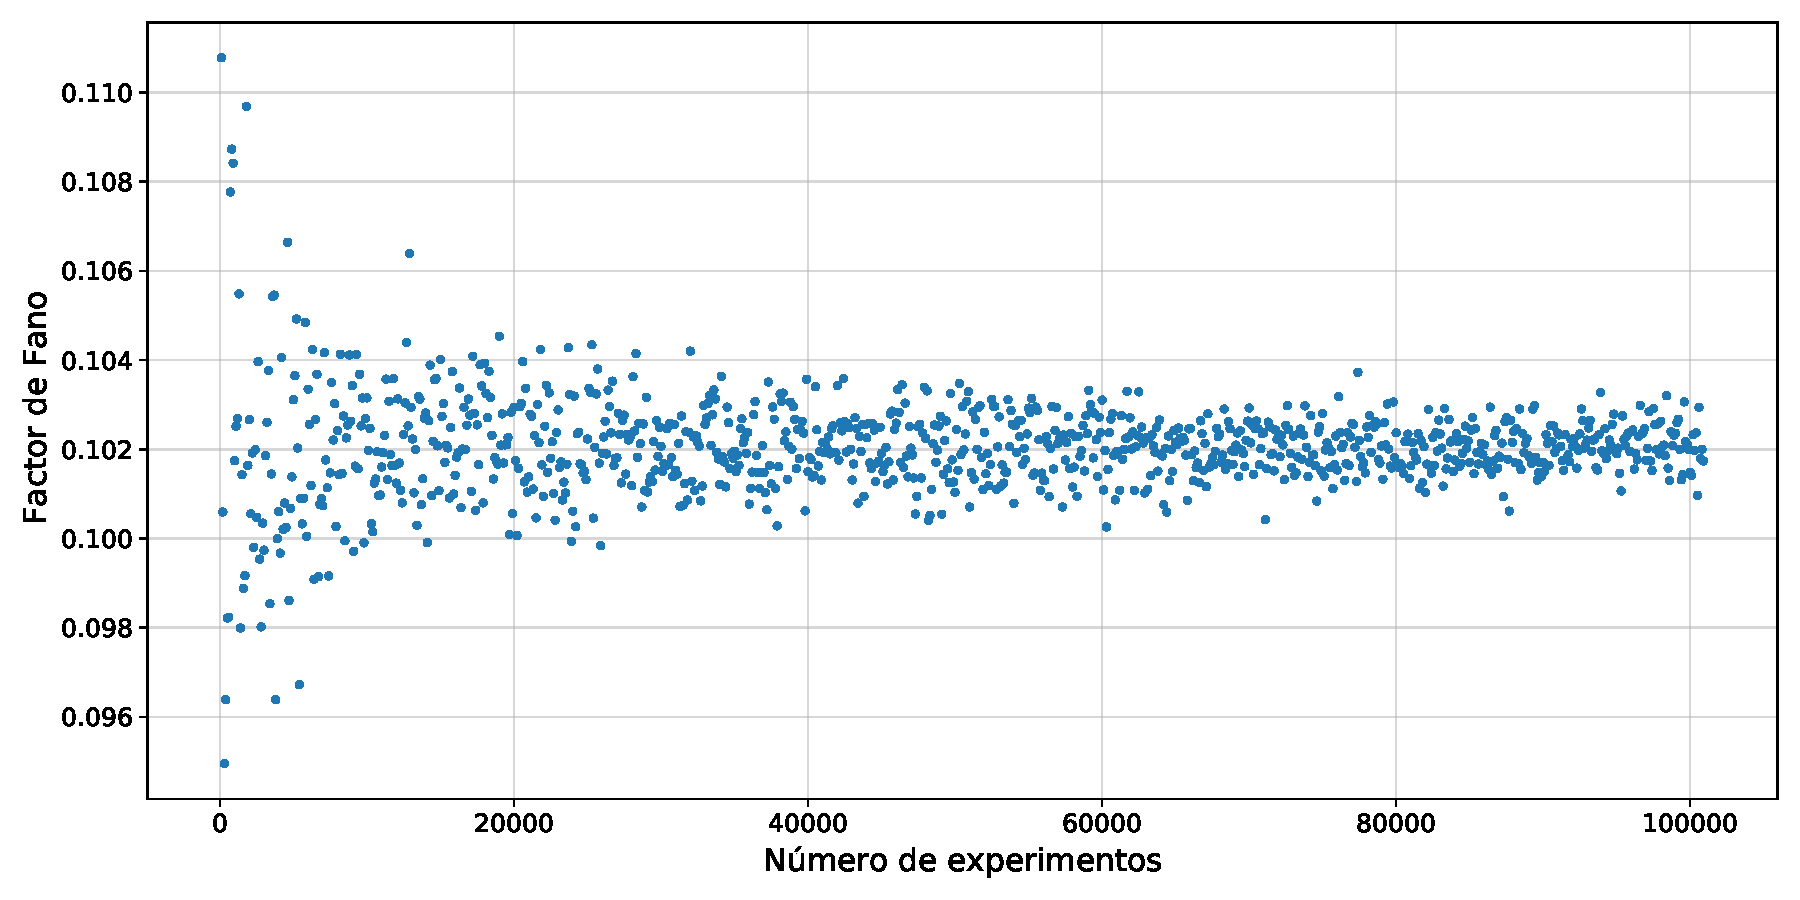
\includegraphics[scale=0.5]{Figs/FanoConvergencia.pdf}
    \caption{Valores del factor de Fano para distintas cantidades de repeticiones del experimento, partiendo desde $100$ repeticiones hasta 100900 repeticiones, utilizando $E_{R} = 677\,\si{eV}$.}
    \label{fig:FanoConvergencia}
\end{figure}
Entre $10^{2}$ y $10^{4}$ repeticiones del experimento se tiene que el factor de Fano se encuentra entre $0.096$ y $0.110$ aproximadamente, mientras que entre $10^{4}$ y $10^{5}$ cantidad de repeticiones los valores para el factor de Fano están acotados entre $\sim 0.100$ y $\sim 0.104$ aproximadamente. Se nota claramente la convergencia de los valores con el aumento de repeticiones y que para $10^{4}$ la variabilidad del factor de Fano es como mucho del $6\%$.

%Se simuló el proceso de cascada con con diferente cantidad de repeticiones, partiendo desde $5000$ hasta incluso $100000$ para asegurar la robustez de la estadística

%Además, con el fin de caracterizar las dependencias entre parámetros en esta implementación particular, se realizaron barridos sobre la pérdida de energía $E_{loss}$ y así conocer la dependencia de los resultados respecto de este, partiendo desde $0\,\si{eV}$ de pérdida de energía hasta $7\,\si{eV}$ de pérdida de energía por cada ionización (equivale a perder casi $4$ veces la energía del gap del silicio). Con esto se quiso observar el comportamiento de esta simulación en este rango de valores, por más que la pérdida de energía final sea demasiado elevada para poder considerarse en el fenómeno físico real. 

%En cada uno de los barridos se obtuvo el factor de Fano, el valor medio de carga ionizada y la energía de creación electrón-hueco, como puede verse en las figuras \ref{fig:FanoVsEloss}, \ref{fig:ElossVsMu} y \ref{fig:CreacionHuecoVsEloss}.
%\begin{figure}%[h]
%a) Esta figura se puede hacer con los datos de: fano_Eloss_mu_vec.txt que está en el directorio /home/igna/Escritorio/Tesis2021/Figs/Figuras_Apendice_Simulaciones/txts_para_plots usando el .py Barridos_mu_Eloss_fano.py que está en /home/igna/Escritorio/Tesis2021/Figs/Figuras_Apendice_Simulaciones/pys_para_plots
%    \centering
%     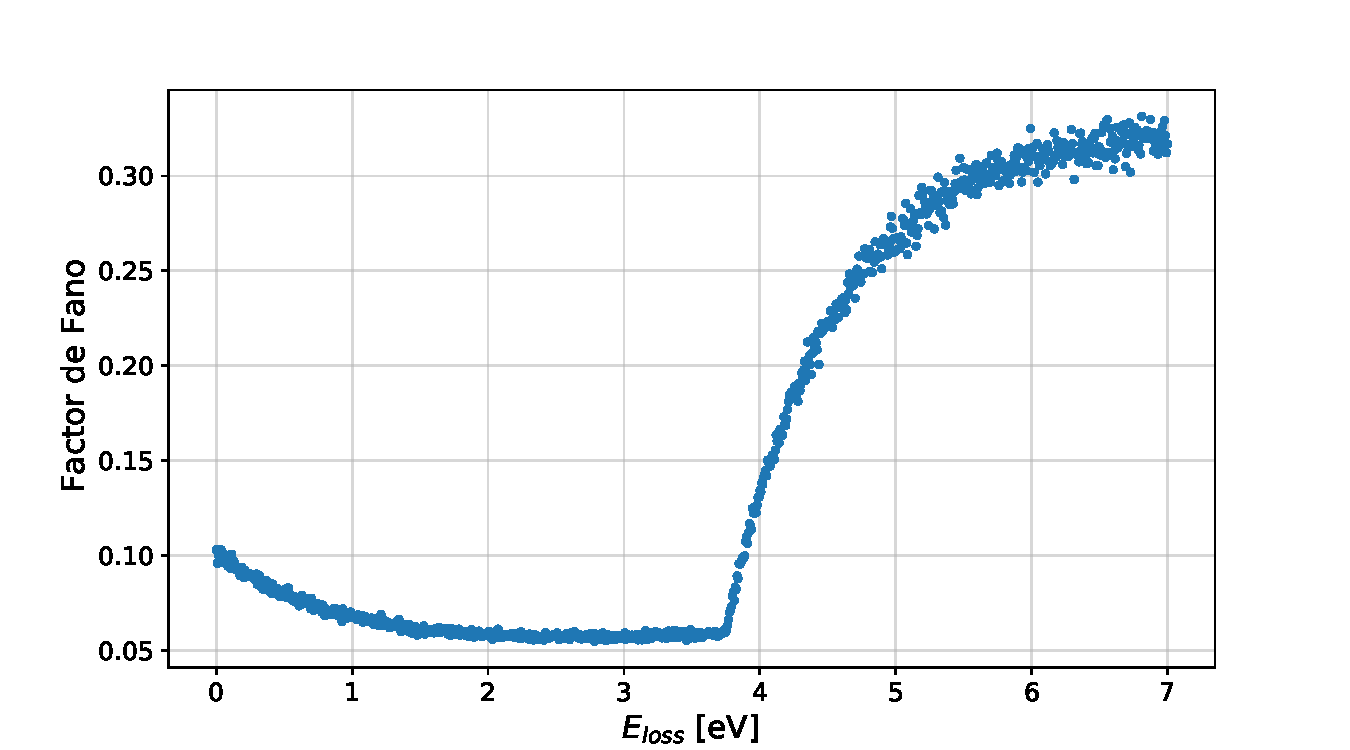
\includegraphics[scale=0.5]{Figs/Fano_vs_Eloss_5ktrials_0-7Eloss.pdf}
%     \caption{\footnotesize{Curva del factor de Fano en función de la energía pérdida por cada ionización. El cambio abrupto en la curva ocurre para $E_{loss} = 3.75\,\si{eV}$, coincidente con la energía media de creación electrón-hueco.}}
%     \label{fig:FanoVsEloss}
% \end{figure}
%La curva del factor de Fano en función de la energía $E_{loss}$ (y al igual que la energía de creación electrón-hueco y el valor medio de carga ionizada) presenta un cambio de régimen abrupto cuando se cruza el umbral $E_{loss} = 3.75\,\si{eV}$. En la Figura \ref{fig:FanoVsEloss} puede verse claramente este cambio de régimen. También se observa que cuando hay conservación de la energía, es decir, $E_{loss} = 0$, es cuando se obtiene un factor de Fano más semejante al observado experimentalmente, que está cerca de $0.1$. A medida que aumenta la pérdida de energía, el factor de Fano comienza a decrecer hasta que se alcanza los $3.75\,\si{eV}$ de pérdida de energía, donde se observa el cambio brusco en la curva, y se observa un aumento pronunciado de la pendiente, semejante a un punto crítico.

%De la misma forma, el valor medio $\mu$ de la carga ionizada tiene un cambio de concavidad en la curva a medida que aumenta la cantidad de energía perdida por cada ionización, como se ve en la Figura \ref{fig:ElossVsMu}.
%\begin{figure}%[h]
% b) Esta figura se puede hacer con los datos de: fano_Eloss_mu_vec.txt que está en el directorio /home/igna/Escritorio/Tesis2021/Figs/Figuras_Apendice_Simulaciones/txts_para_plots usando el .py Barridos_mu_Eloss_fano.py que está en /home/igna/Escritorio/Tesis2021/Figs/Figuras_Apendice_Simulaciones/pys_para_plots
%     \centering
%     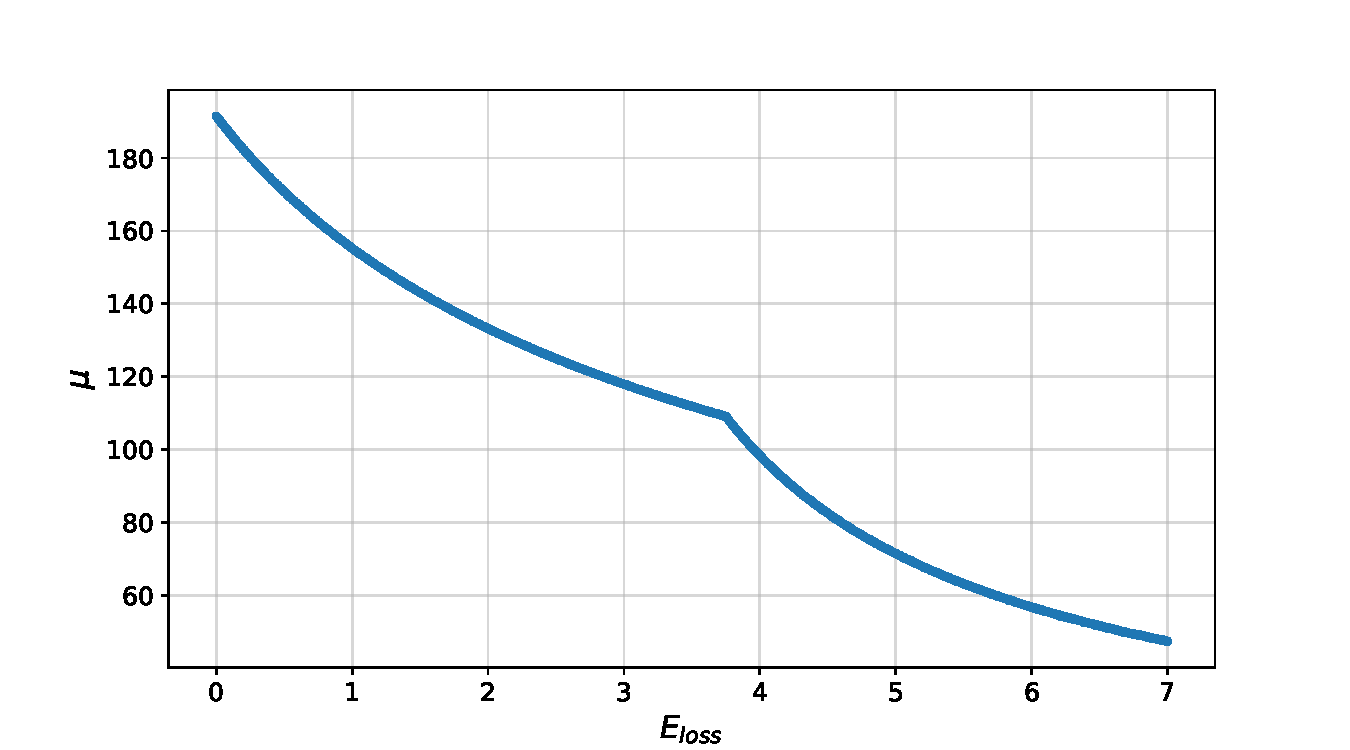
\includegraphics[scale=0.5]{Figs/ELoss_vs_mu_5ktrials_0-7Eloss.pdf}
%     \caption{\footnotesize{Curva del valor medio de carga $\mu$ en función de la energía perdida por cada ionización. El cambio abrupto en la curva ocurre para $E_{loss} = 3.75\,si{eV}$, coincidente con la energía media de creación electrón-hueco.}}
%     \label{fig:ElossVsMu}
% \end{figure}
%Nuevamente, los valores más cercanos a los medidos experimentalmente son los que corresponden a los casos en los que no hay disipación de energía.

%Por último, para la energía de creación electrón-hueco, calculada a partir del valor medio de carga ionizada y la energía inicial $E_{R} = 677\,\si{eV}$, usando que $\mean{\varepsilon_{\eh}} = 677\,\si{eV}/\mu$, es claro que esta tendrá el mismo cambio de régimen en $3.75\,\si{eV}$, como se ve en la Figura \ref{fig:CreacionHuecoVsEloss}.
%\begin{figure}%[h]
%a) Esta figura se puede hacer con los datos de: fano_Eloss_mu_vec.txt que está en el directorio /home/igna/Escritorio/Tesis2021/Figs/Figuras_Apendice_Simulaciones/txts_para_plots usando el .py Barridos_mu_Eloss_fano.py que está en /home/igna/Escritorio/Tesis2021/Figs/Figuras_Apendice_Simulaciones/pys_para_plots
%     \centering
%     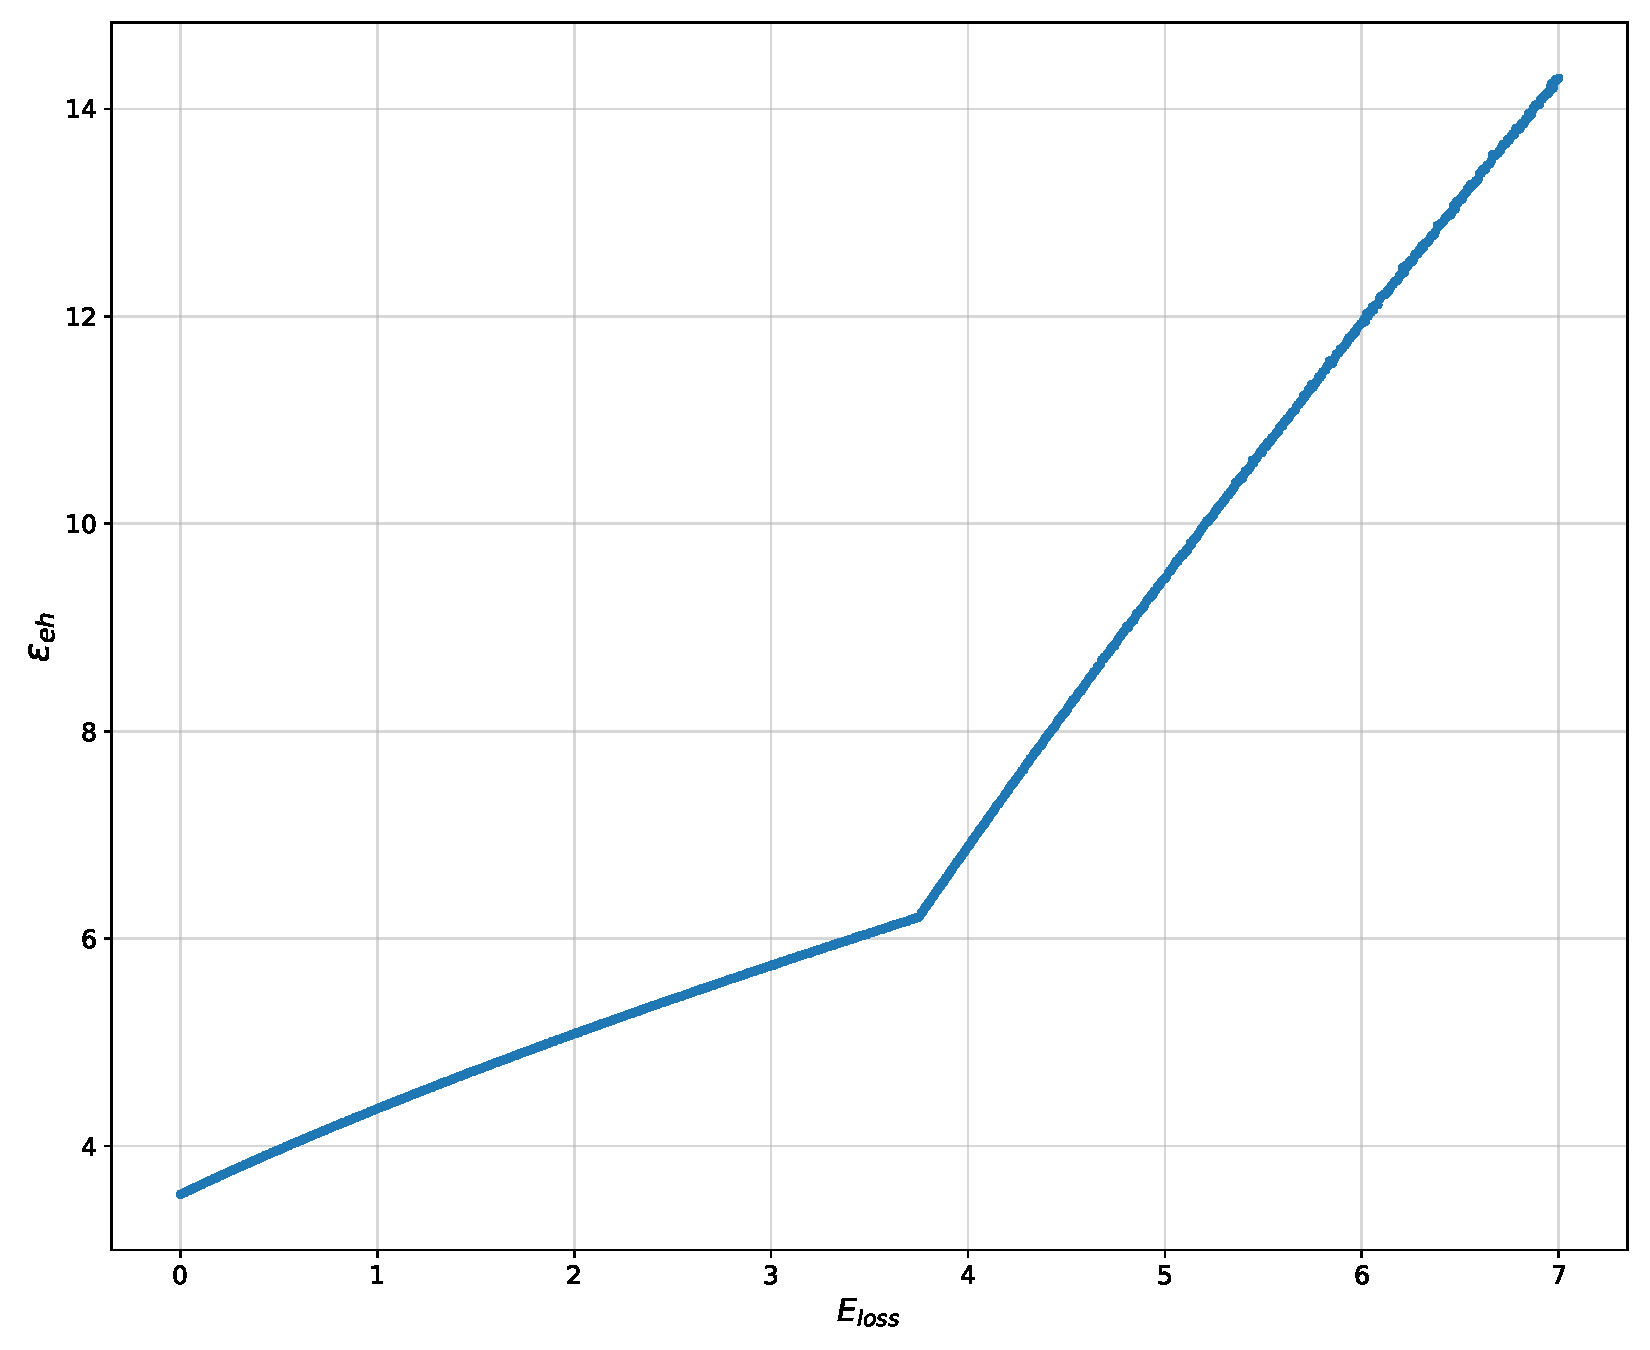
\includegraphics[scale=0.5]{Figs/E_eh_vs_Eloss_5ktrials_0-7Eloss.pdf}
%     \caption{\footnotesize{Curva del valor medio de la energía de creación de electrón-hueco en función de la energía perdida por cada ionización. El cambio abrupto en la curva ocurre para $E_{loss} = 3.75\,si{eV}$, coincidente con la energía media de creación electrón-hueco. Esta curva se obtiene utilizando el valor medio de carga ionizada $\mu$ y la energía inicial $677\,\si{eV}$.}}
%     \label{fig:CreacionHuecoVsEloss}
% \end{figure}
%Con lo cual se observa que este Monte Carlo es muy sensible a dos parámetros muy importantes de la física real del sistema: La energía de creación electrón-hueco, que es el parámetro de la simulación que determina si hay o no ionización\footnote{Como se verá en el apéndice}; y la conservación de la energía.%Se observa que cuando la energía se conserva en la simulación, se obtienen los resultados más cercanos a los observados experimentalmente y reportados en la bibliografía.
%Con estos barridos se vio la dependencia de tanto del factor de Fano, como de la energía de creación electrón-hueco y del valor medio de carga ionizada al variar el valor de la energía que se pierde con cada ionización. Se observó que estos parámetros son muy sensibles a la pérdida de energía del sistema, obteniéndose resultados con cambios de regímenes muy pronunciados, particularmente, cuando la energía perdida por ionización coincide con el valor $E_{loss} = 3.75\,\si{eV}$, que casualmente es la energía de creación electrón-hueco promedio y que se usó en la simulación como un parámetro fijo dentro del código, como se verá en el apéndice \ref{app:Implementación}.

%En cuanto a los resultados de las simulaciones del factor de Fano, se realizaron simulaciones tanto para la energía de los rayos $X$ del flúor como para la de los rayos $X$ del aluminio, de $677\,\si{eV}$ y $1500\,\si{eV}$ respectivamente.

En cuanto a los resultados de estas simulaciones, para el caso del flúor, se pueden ver los histogramas de carga en los gráficos de las figuras \ref{fig:F_fano_A5.2} y \ref{fig:F_fano_A20}. Ambos gráficos fueron realizados con $100000$ repeticiones del experimento, pero con distintos valores del parámetro $A$. En estos se muestra la distribución de carga con un ajuste gaussiano, del cual se deriva el valor de $\mu$ posteriormente utilizado para graficar una curva poissoniana. En ambos casos se observa como la distribución de carga está lejos de parecerse a una distribución de Poisson y por ello el factor de Fano se aleja de la unidad. En la Figura \ref{fig:F_fano_A5.2} se puede ver que una distribución gaussiana es una buena descripción del histograma. En este caso se utilizó $A = 5.2\,\si{eV}^{3}$, el factor de Fano corresponde a $F = 0.1018 \pm 0.0004$ y el valor medio de carga $\mu = 191.50 \pm 0.01$, un valor significativamente mayor que el valor esperado, cercano a $\mu = 181$.
\begin{figure}[h]
%Los datos para este gráfico están en /home/igna/Escritorio/Tesis2021/Figs/Figuras_Apendice_Simulaciones/txts_para_plot F_E677_A5.2_E_loss0_Trials100000.txt Para modificar el graf hay que correr el .py que están en /home/igna/Escritorio/Tesis2021/Figs/Figuras_Apendice_Simulaciones/pys_para_plots: Al_Fano_E1570_A5.2_trials100k_histcarga.py
    \centering
    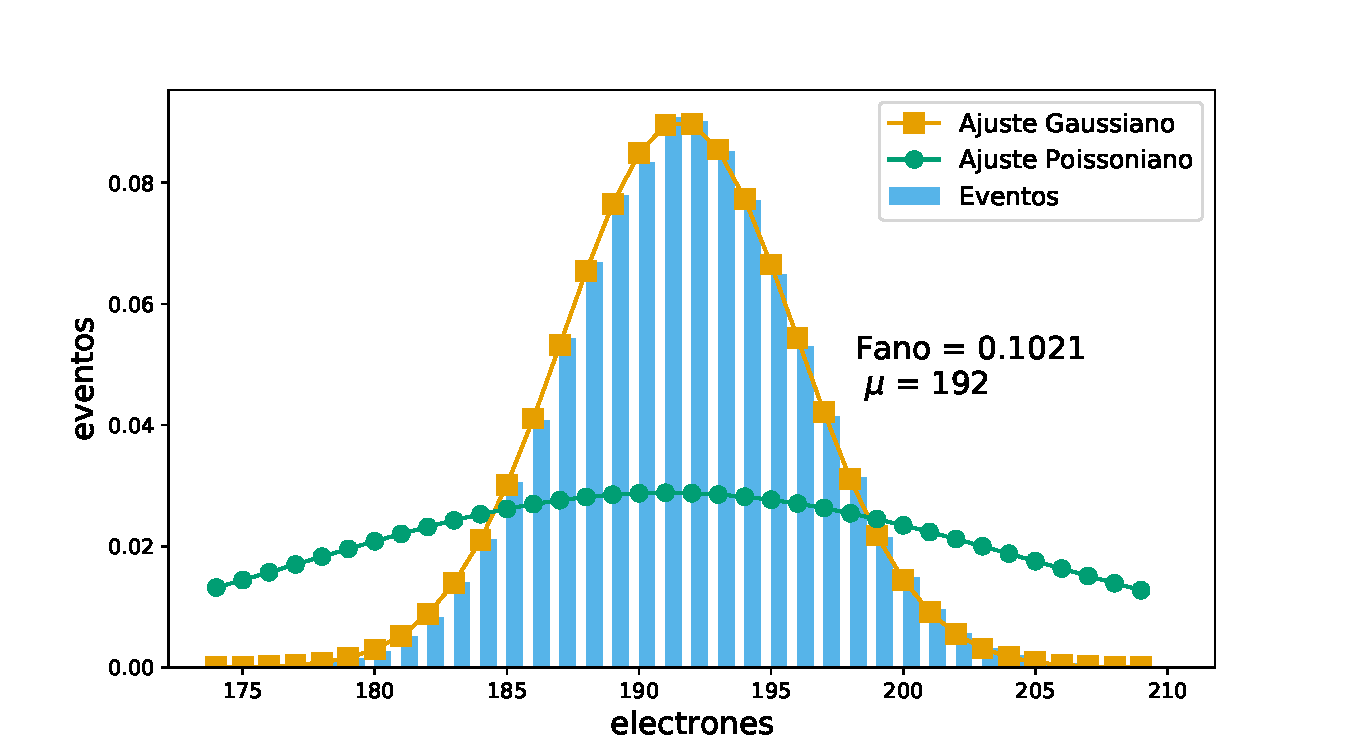
\includegraphics[scale=0.5]{Figs/F_Fano_E677_A5.2_Eloss0_100ktrials.pdf}
    \caption{Distribución de carga simulada con el método de Monte Carlo, con parámetro $A = 5.2\,\si{eV}^{3}$ y $10^{5}$ repeticiones del experimento. Se observa un valor medio $\mu = 191.50 \pm 0.01$, lo cual representa un corrimiento hacia la derecha del valor esperado para el pico de los rayos $X$ del flúor, que es alrededor de $181$ electrones un valor del factor de Fano de $F = 0.1018 \pm 0.0004$.}
    \label{fig:F_fano_A5.2}
\end{figure}
\noindent Para el segundo caso, en la Figura \ref{fig:F_fano_A20}, se modificó el valor del parámetro $A$ hasta que el pico coincida con el valor medio de carga esperado, y su valor fue $\mu = 181.12 \pm 0.02$ electrones. El valor de $A$ que cumple esa condición es $A = 20\,\si{eV}^{3}$, valor $5$ veces mayor al propuesto en la bibliografía para describir macroscópicamente las propiedades del silicio.
\begin{figure}[h]
%Los datos para este gráfico están en /home/igna/Escritorio/Tesis2021/Figs/Figuras_Apendice_Simulaciones/txts_para_plot F_E677_A20_E_loss0_Trials100000.txt Para modificar el graf hay que correr el .py que están en /home/igna/Escritorio/Tesis2021/Figs/Figuras_Apendice_Simulaciones/pys_para_plots: Al_Fano_E1570_A20_trials100k_histcarga.py
    \centering
    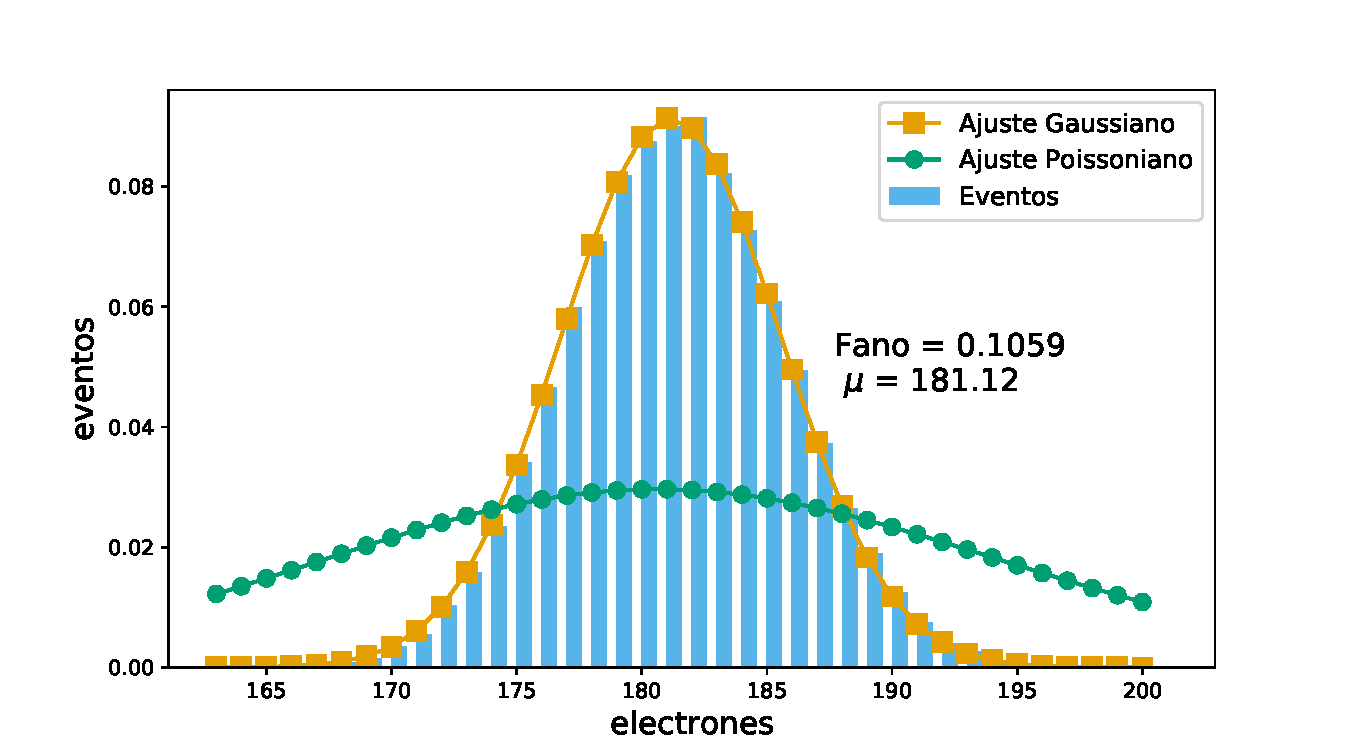
\includegraphics[scale=0.5]{Figs/F_Fano_E677_A20_Eloss0_100ktrials.pdf}
    \caption{Distribución de carga simulada con el método de Monte Carlo, forzando el parámetro $A$ para que el pico se encuentre en los $181.12 \pm 0.02$ electrones esperados para los $677\,\si{eV}$ de energía de los rayos X del flúor. El valor necesario para esto suceda fue $A=20\,\si{eV}^{3}$ y el factor de Fano obtenido fue $F = 0.1059 \pm 0.0004$.}
    \label{fig:F_fano_A20}
\end{figure}
El factor de Fano en este caso es de $F = 0.1059 \pm 0.0004$, que está contenido entre las bandas esperadas para la cantidad de estadística utilizada en esta simulación, al igual que para el caso anterior.

De la misma manera que para la energía del flúor, se presentan los resultados para las simulaciones para los rayos $X$ del aluminio en las Figuras \ref{fig:Al_fano_A5.2} y \ref{fig:Al_fano_A22}. Los resultados son muy similares a los del flúor. En ambos gráficos puede verse como las curvas de Poisson correspondientes al $\mu$ obtenido de las simulaciones difiere fuertemente de los histogramas, mientras que los ajustes gaussianos se encuentran en muy buen acuerdo con ellos. 
\begin{figure}[h]
%Los datos para este gráfico están en /home/igna/Escritorio/Tesis2021/Figs/Figuras_Apendice_Simulaciones Para modificar el graf hay que correr el .py que están en /home/igna/Escritorio/Tesis2021/Figs/Figuras_Apendice_Simulaciones/pys_para_plots
    \centering
    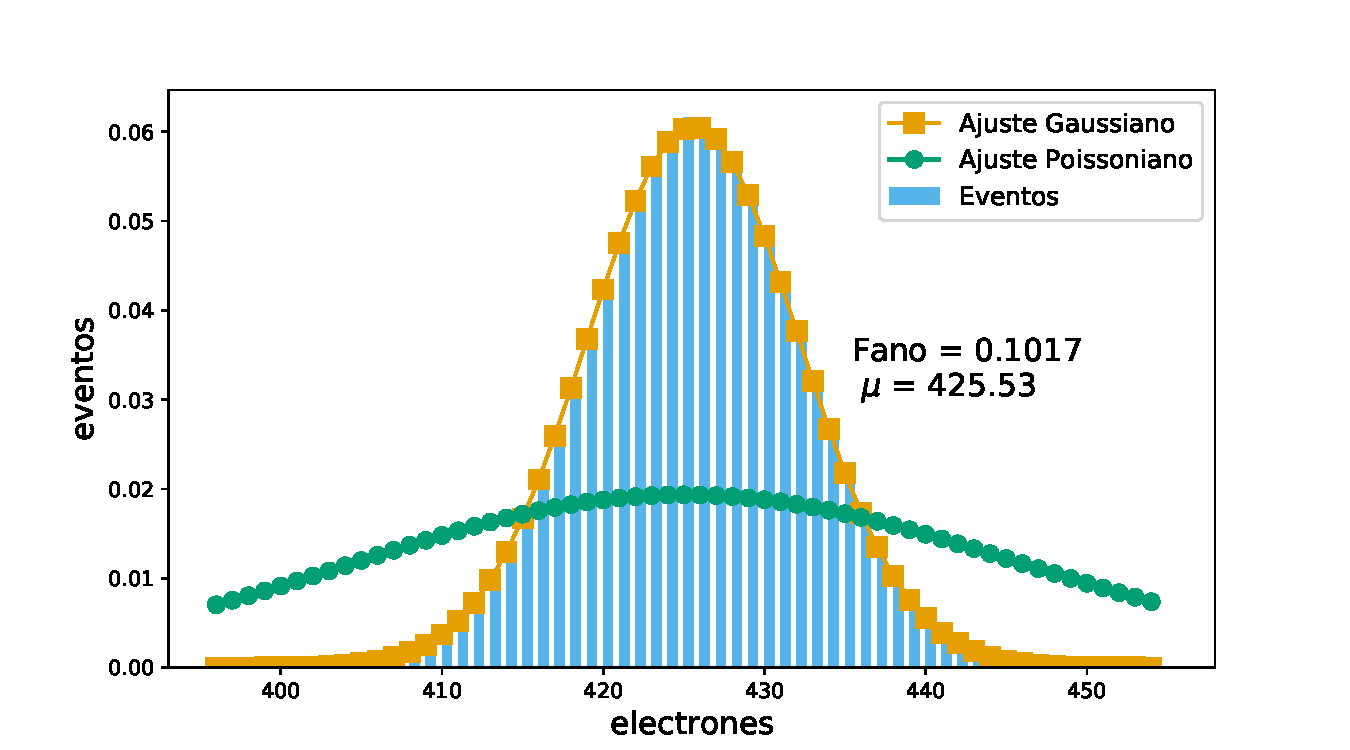
\includegraphics[scale=0.5]{Figs/Al_Fano_1500_A5.2_Eloss0_100ktrials.pdf}
    \caption{Distribución de carga simulada con el método de Monte Carlo, con parámetro $A = 5.2\,\si{eV}^{3}$ y $10^{5}$ repeticiones del experimento. Se observa un valor medio $\mu = 425.53 \pm 0.02$, lo cual representa un corrimiento hacia la derecha del valor esperado para el pico de los rayos $X$ del aluminio, que es alrededor de $400$ electrones. Se obtuvo un factor de Fano $F = 0.1017 \pm 0.0003$.}
    \label{fig:Al_fano_A5.2}
\end{figure}

En la Figura \ref{fig:Al_fano_A5.2} se simuló el proceso partiendo de $E_{R} = 1500\,\si{eV}$, con $100000$ repeticiones del experimento y $A = 5.2\,\si{eV}^{3}$ como indica la bibliografía. Sin embargo, el valor medio de carga esperado presenta nuevamente un corrimiento hacia la derecha, teniéndose $\mu = 425.53 \pm 0.02$ y un factor de Fano $F = 0.1017 \pm 0.0003$.

Por último, en la Figura \ref{fig:Al_fano_A22} se repitió la simulación variando $A$ hasta obtener el un valor medio de carga semejante al esperado. Con $A = 22\,\si{eV}^{3}$ se obtuvo $\mu = 400.28 \pm 0.02$. El factor de Fano en este caso resultó $F = 0.1054 \pm 0.0004$, también contenido entre los valores esperados, como se vio en la Figura \ref{fig:FanoConvergencia}.

Tanto para el caso del flúor como para el caso del aluminio se observaron valores del factor de Fano muy semejantes entre sí, con lo cual parecería que para esta implementación de la simulación Monte Carlo, la energía inicial $E_{R}$ no resulta ser un parámetro relevante para esta magnitud.
\begin{figure}[h]
%Los datos para este gráfico están en /home/igna/Escritorio/Tesis2021/Figs/Figuras_Apendice_Simulaciones/txts_para_plots. Para modificar el graf hay que correr el .py que están en /home/igna/Escritorio/Tesis2021/Figs/Figuras_Apendice_Simulaciones/pys_para_plots
    \centering
    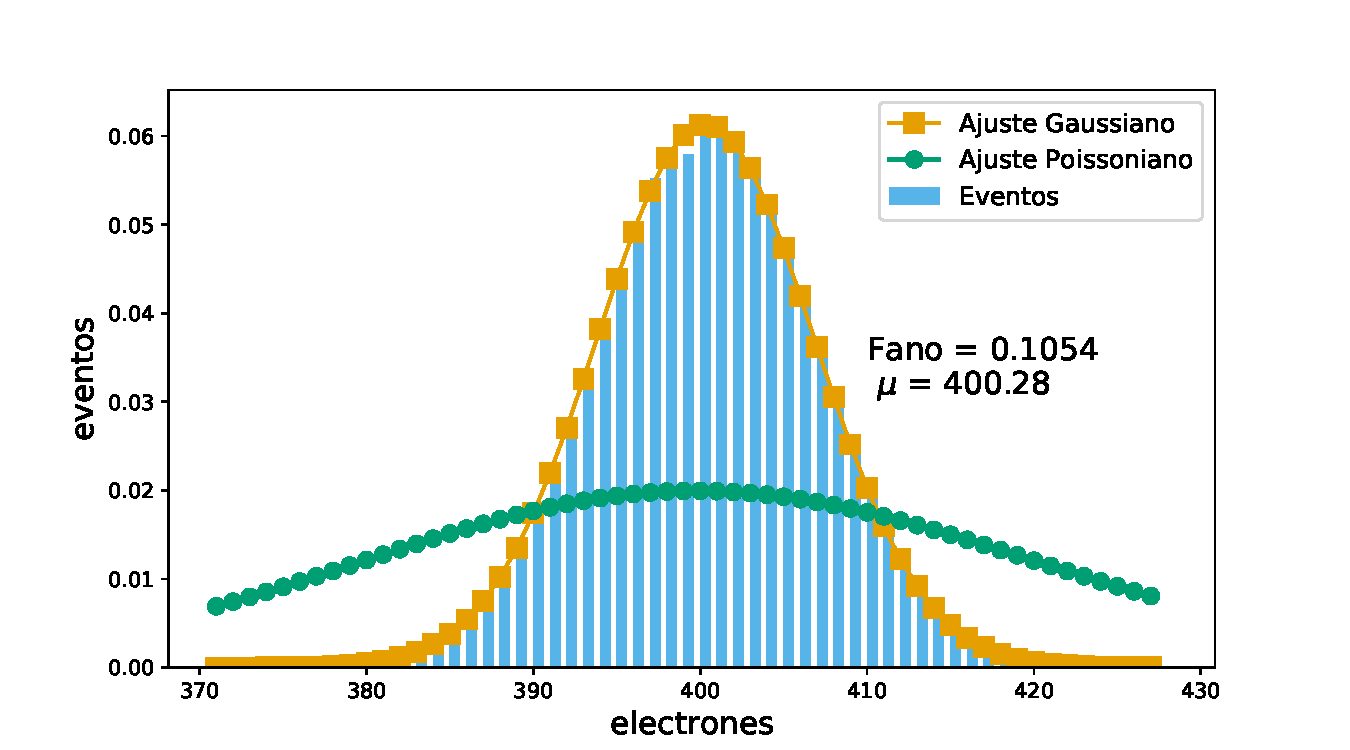
\includegraphics[scale=0.5]{Figs/Al_Fano_1500_A22.0_Eloss0_100ktrials.pdf}
    \caption{Distribución de carga simulada con el método de Monte Carlo, forzando el parámetro $A$ para que el pico se encuentre en los $400.28 \pm 0.02 $ electrones esperados para los $1500\,\si{eV}$ de energía de los rayos X del aluminio. El valor necesario para esto suceda fue $A=22\,\si{eV}^{3}$ y el factor de Fano obtenido $F = 0.1054 \pm 0.0004$.}
    \label{fig:Al_fano_A22}
\end{figure}
Además se obtuvieron valores cercanos a los reportados en diferentes trabajos\cite{Ryan, Alig, Janesick2, Fraser, Owens} tanto por medio de simulaciones como por mediciones.

De estas simulaciones se esperaba poder comprender mejor una de las posibles razones de por qué el factor de Fano es menor a la unidad en las mediciones experimentales. La hipótesis que sustentan las simulaciones es que el proceso pierde su carácter poissoniano por depositarse toda la energía en el interior del material y que una fracción de ella no se utiliza para ionizar sino para producir fonones.
